\chapter{Convolutional Neural Networks}

Le \textbf{Convulutional Neural Network} (CNN) sono ispirate dal funzionamento dell'organizzazione della corteccia visiva animale: così come il nostro cervello riconosce volti, forme, oggetti a partire da stimoli visivi grezzi, le CNN imparano a rilevare caratteristiche visive come bordi, texture e forme, combinandole per riconoscere oggetti più complessi. Le reti neurali che noi conosciamo bene, solo quelle completamente connesse, esse non sono adatte per elaborare delle immagini grandi. Se consideriamo il dataset \textbf{CIFAR-10}, le immagini al suo interno sono 32x32x3 (32 pixel larghe, 32 pixel alte e 3 canali di colore), pertanto se dovessimo considerare una rete neurale completamente connessa, essa avrebbe nel suo primo layer ben 3072 pesi per un singolo neurone, il che è un numero fattibile, ma notevolmente elevato. Nel momento in cui ci si sposta a immagini con dimensioni più grandi, per esempio un'immagine 200x200x3 avrò ben 120.000 pesi per ogni singolo neurone. Possiamo notare come questo sia uno spreco, e ci porterà con gran probablità all'overfitting e un'inefficienza computazionale. La grande forza delle reti convoluzionali risiede nella ricezione degli input poiché li tratta come un volume tridimensionale, essi infatti aderiscono molto meglio con questa architettura, poiché ha unità che garantiscono ben tre dimensioni (Larghezza, Altezza e Profondità), e ogni layer permette di produrre un nuovo volume tridimensionale chiamato \textit{Activation Volume}. Ogni neurone a differenza della \textit{fully connected} è connesso solo a una porzione locale dello spazio, chiamata \textit{receptive field}, il valore dell'estensione di questo campo di connettività è un iperparametro.
\begin{Osservazione}
    L'estensione della connettività lungo l'asse della profondità è sempre uguale alla profondità del volume di input. Pertanto è importante sottolineare questa asimmetria nel trattamento delle dimensioni spaziali, la cui è completa lungo la profondità ma parziale sulle altre.
\end{Osservazione}

\begin{figure}
    \centering
    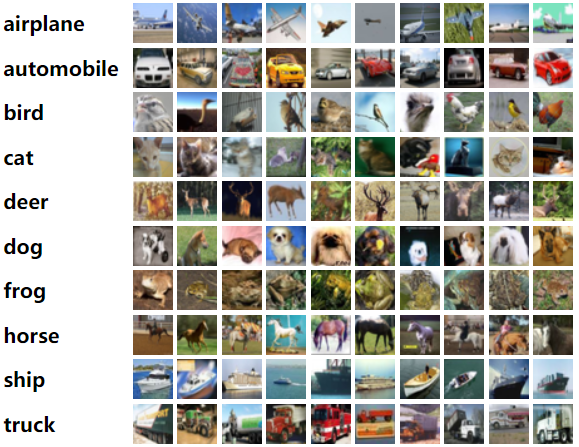
\includegraphics[width=0.40\linewidth]{figure/Cifar_dataset.png}
    \caption{Rappresentazione di una piccola parte del Cifar Dataset, un dataset che contiene una delle collezioni di immagini più utilizzate nel campo del deep learning e della computer vision, particolarmente per l’addestramento e la valutazione di reti neurali.}
    \label{fig:cifar_ds}
\end{figure}

\section{Analisi dell'architettura}
La rete convoluzionale è sviluppata diversamente da quelle viste precedentemente, poiché è suddivisa in diversi livelli, i quali si occupano di manipolazioni dei dati in maniere differenti e di volta in volta vi è: uno strato convoluzionale, uno strato di attivazione, uno strato di polling e uno strato completamente connesso che viene posto solitamente a conclusione della rete. Le \textbf{CNN}, applicano dei filtri, che possono essere immaginati come dei piccoli parallelepipedi i quali hanno il compito di concentrarsi su una specifica caratteristica dell'immagine, il filtro scorre attraverso l'altezza e la larghezza della nostra immagine e apporta una convoluzione delle due, ottenendo un risultato, generando una mappa di attivazione (Figura~\ref{fig:convolution_layer}).

\begin{figure}[htbp]
    \centering
    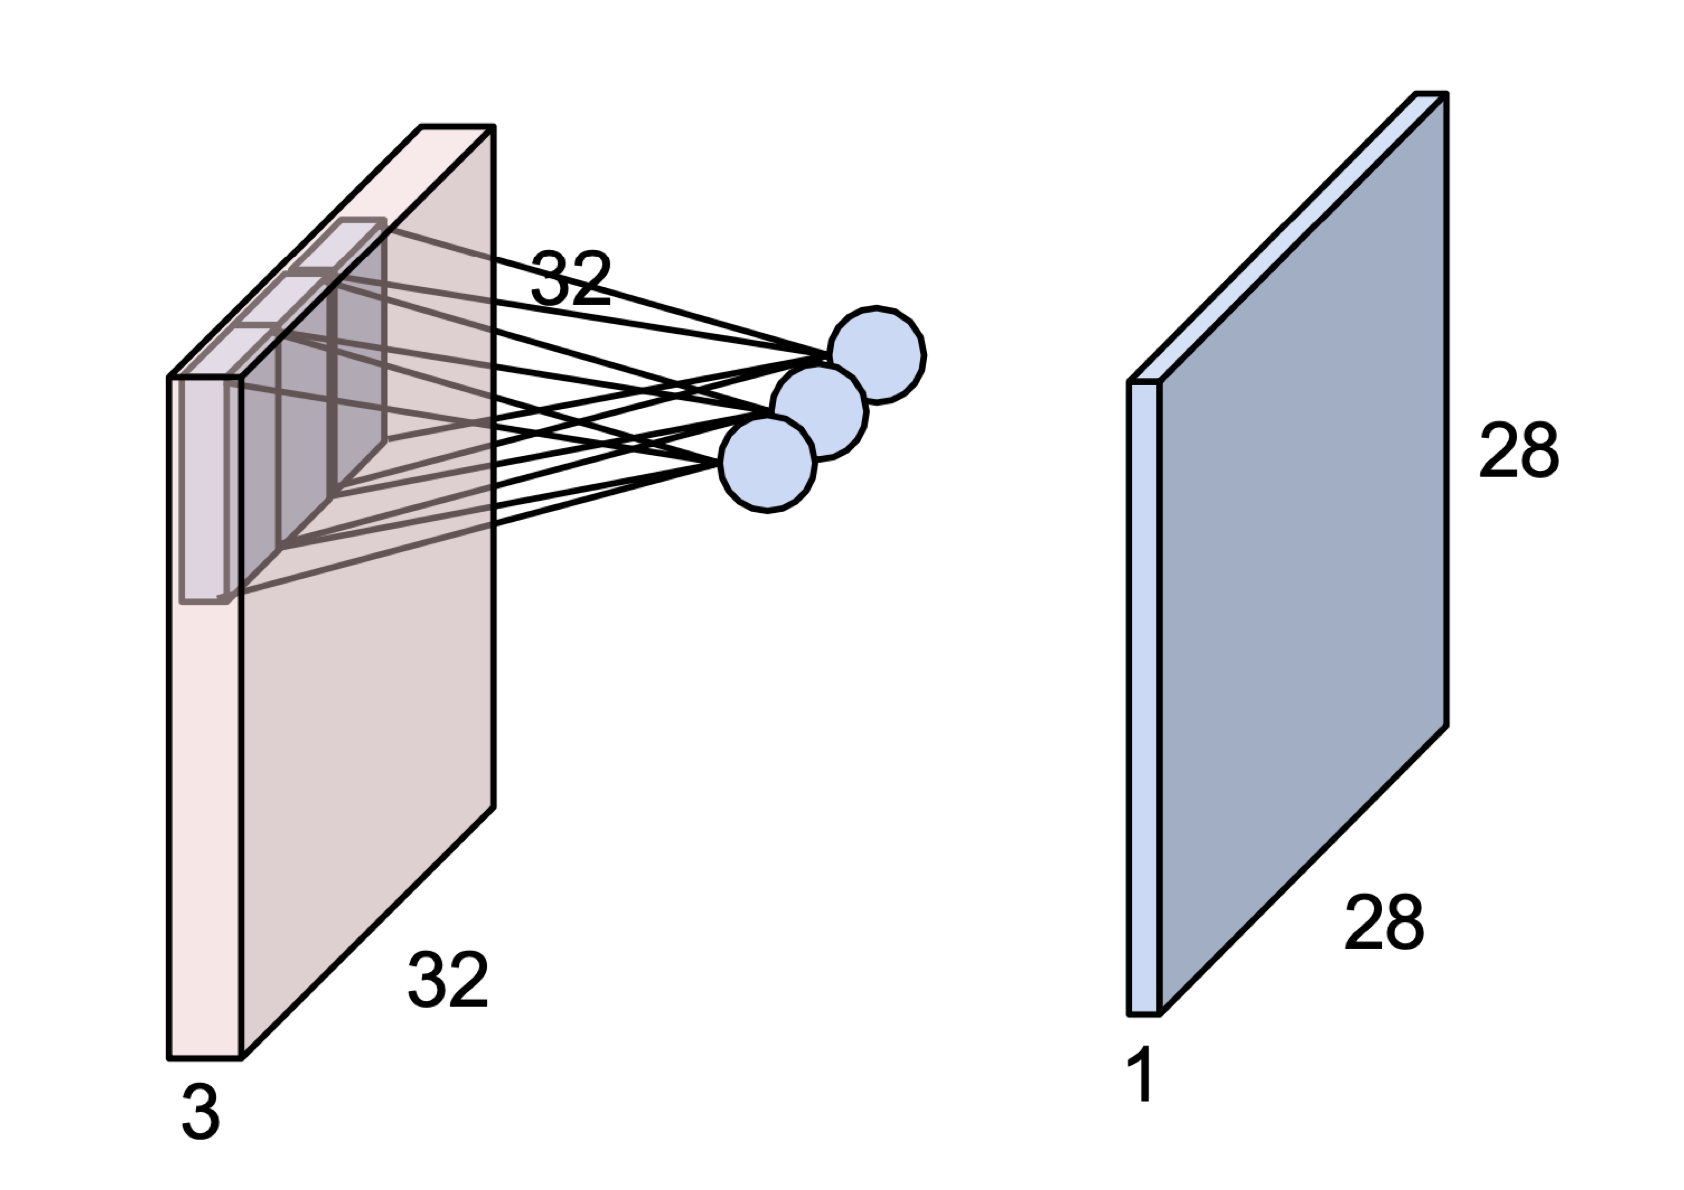
\includegraphics[width=0.55\textwidth]{figure/CNNConv.png}
    \caption{A sinistra abbiamo la rappresentazione intera dei nostri input al quale vengono applicati dei filtri, i piccolo parallelepipedi blu, i quali generano degli output, che poi una volta applicati a tutti gli input, portano alla creazione dell'activation layer, visibile in figura sulla destra.}
    \label{fig:convolution_layer}
\end{figure}

Se dovessimo limitarci esclusivamente a una singola caratteristica la rappresentazione presente in Figura~\ref{fig:convolution_layer}, ci potrebbe persino bastare. Per avere un efficiente riconoscitore d'immagine si utilizzano però più filtri compattati, come se fossero un unico filtro, in modo tale da ottenere un'analisi più approfondita, ottenendo ciò che è visibile in figura~\ref{fig:convolution_layer_multifilter}, prima di generare lo strato di attivazione vi è un'attivazione dei gli output ottenuti dallo strato di convoluzione, solitamente viene utilizzata la funzione \textbf{ReLU}, ma ovviamente al posto di questa possiamo utilizzare una qualunque delle funzioni di attivazione precedentemente citate nel capitolo~\ref{chpt:5}.


\begin{figure}[htbp]
    \centering
    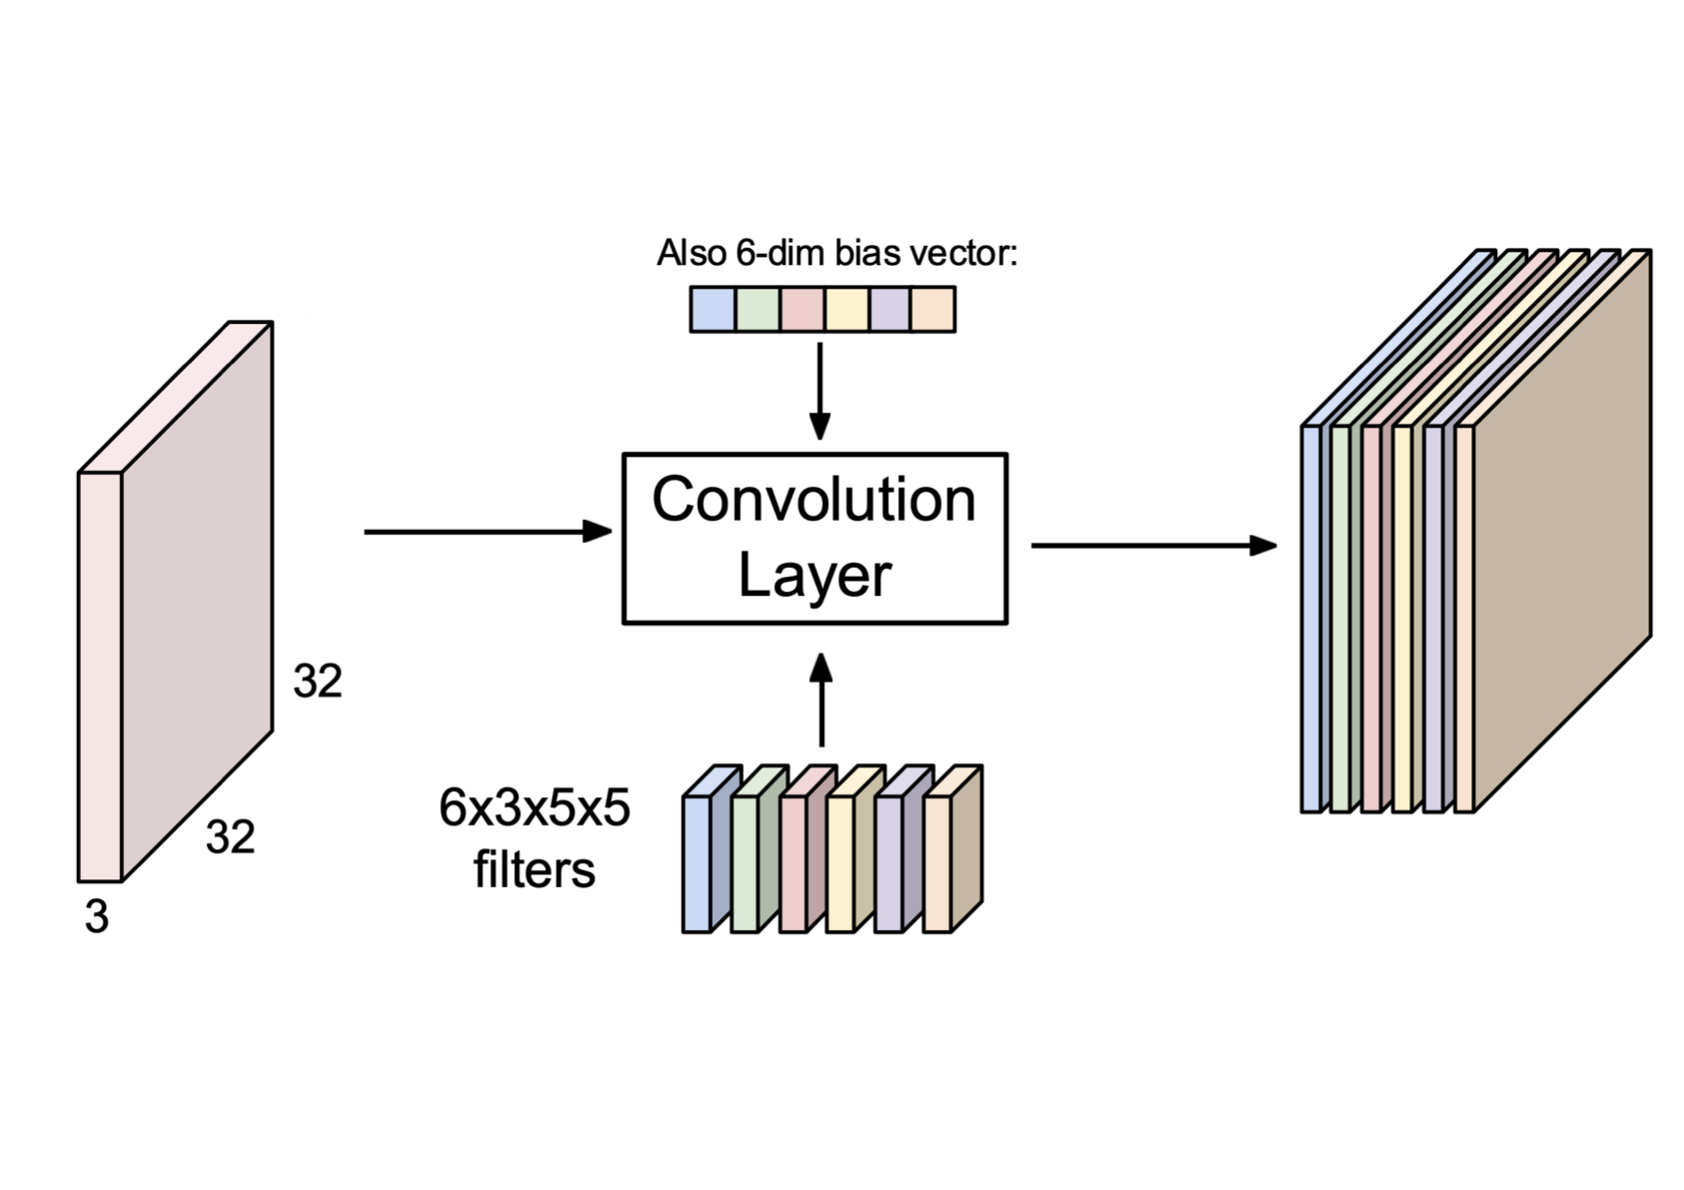
\includegraphics[width=0.85\textwidth]{figure/CNNConvolution2.png}
    \caption{Viene applicata la convoluzione con un multi filtro che permette di rilevare più feature in un'unica volta, il quale ci genera uno stack di attivazione più profondo, di quello di partenza, ma con dimensioni ridotte nelle altre dimensioni.}
    \label{fig:convolution_layer_multifilter}
\end{figure}

\section{Il filtro e le sue caratteristiche}

Quando analizziamo le reti convoluzionali, abbiamo visto che ci sono diversi layer, i quali si occupano di cose differenti. Adesso però soffermiamoci particolarmente su un layer, ma ancor più nello specifico in una parte della costituzione di un layer, ossia il filtro. Esso infatti può essere utilizzato in diverse maniere, per poter estrarre il layer di attivazione, la decisione della dimensionalità del filtro non è effettuata a caso, ma deve essere opportunatamente scelta in base alla dimensione dell'input layer. Una caratteristica del filtro molto importante da considerare, è il passo con cui esso scorre al di sopra del nostro input layer, ossia di quanto si discosta una volta che ho applicato il filtro la prima volta prima di essere applicato una seconda (Figura~\ref{fig:filter_stride}). 
\begin{figure}
    \centering
    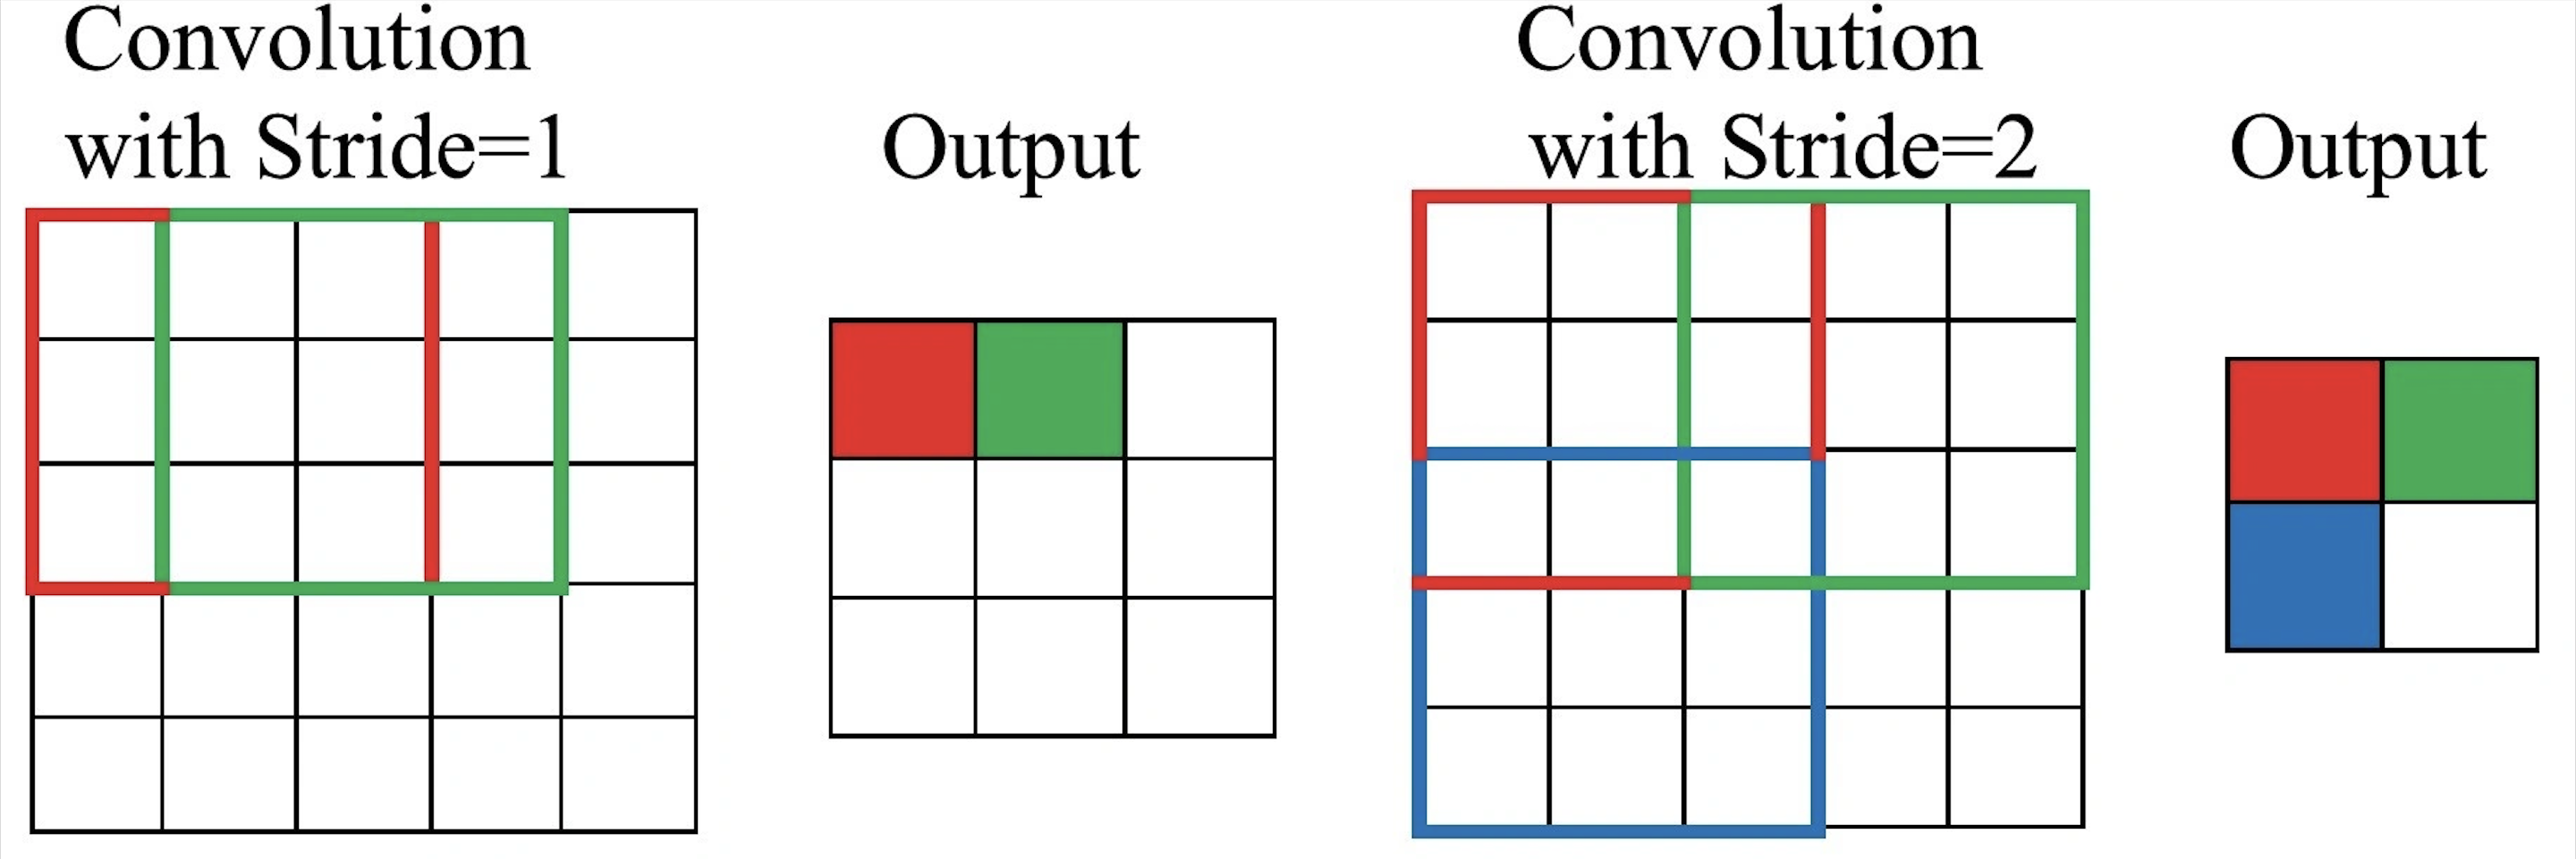
\includegraphics[width=0.90\textwidth]{figure/Filtering_stride.png}
    \caption{Applicazione di un filtro a uno stesso input layer, con a sinistra uno passo di uno, mentre a destra con un passo di due, generando a un output layer di dimensionalità differente.}
    \label{fig:filter_stride}
\end{figure}

Per calcolare invece la dimensione dell'output, si utilizza una semplice equazione, la quale tiene conto della dimensione dell'input ($N$), la dimensione del filtro ($F$) e la dimensione dello stride utilizzato ($S$).

\begin{equation}
    Output = \frac{N-F}{S} + 1
\end{equation}

Nella pratica invece, viene aggiunto un padding intorno al nostro input layer, prima ancora che venga applicato il filtro con il suo stride. Questo avviene perché, nel momento in cui andiamo ad applicare il filtro, privato di questo padding, riceveremo un rimpicciolimento dell'immagine, che in realtà è il nostro scopo reale, tuttavia dopo numerosi strati l'immagine giunge a delle dimensioni molto ridotte, pertanto non risulta più una riduzione efficiente. Se non applicassimo il padding, i pixel posti ai bordi verrebbero utilizzati molto meno nel calcolo della convoluzione, invece con il padding, tutti i pixel partecipano con la stessa frequenza e importanza a ogni convoluzione. Non utilizzare il padding inoltre, porterebbe a una perdita d'informazione, poiché viene tagliata la parte più esterna dell'immagine, mentre utilizzandolo si conserverebbe più contesto visivo. L'equazione della dimensione dell'otuput pertanto si modifica nel seguente modo:

\begin{equation}
    Output = \frac{N+2P-F}{S} +1
\end{equation}

\subsection{Filtri 1x1}

I filtri 1x1 nelle reti neurali convoluzionali (CNN) possono sembrare controintuitivi, ma svolgono ruoli fondamentali nell'ottimizzazione e nella potenza espressiva delle reti. Un filtro 1x1 applica una convoluzione su ogni singolo pixel, considerando però tutti i canali (es. R, G, B) contemporaneamente. Non modifica la dimensione spaziale (altezza e larghezza), ma agisce sulla profondità (numero di canali). Esso può servire per:

\begin{itemize}
    \item \textbf{Riduzione della dimensionalità}: Un filtro 1×1 può ridurre il numero di canali, diminuendo così i parametri e i costi computazionali. Ad esempio, da 256 canali a 64;
    \item \textbf{Aumento della dimensionalità}: Al contrario, può aumentare i canali per arricchire la rappresentazione dei dati;
    \item \textbf{Aggiunta di non linearità}: Combinato con funzioni di attivazione (es. ReLU), introduce non-linearità, migliorando la capacità di apprendimento della rete;
    \item \textbf{Interazione tra canali}: Permette di combinare informazioni tra diversi canali, facilitando l'apprendimento di caratteristiche complesse.
\end{itemize}


\section{Receptive Fields Estesi}

Il Receptive Field (campo recettivo) è la porzione dell’immagine originale che influenza l’attivazione di un singolo neurone in uno specifico strato. Più si va in profondità nella rete, più il campo visivo del neurone si espande: cominciando a vedere regioni più grandi dell'immagine (Figura~\ref{fig:recp_field}). Questo perché nel momento in cui mi muovo in un layer più profondo oltre a visualizzare alcuni neuroni, vedrò anche ciò che vedono i singoli neuroni a loro volta, e per questo espandero il mio campo recettivo, avendo una visione di insieme, sempre più espansa.
\begin{figure}
    \centering
    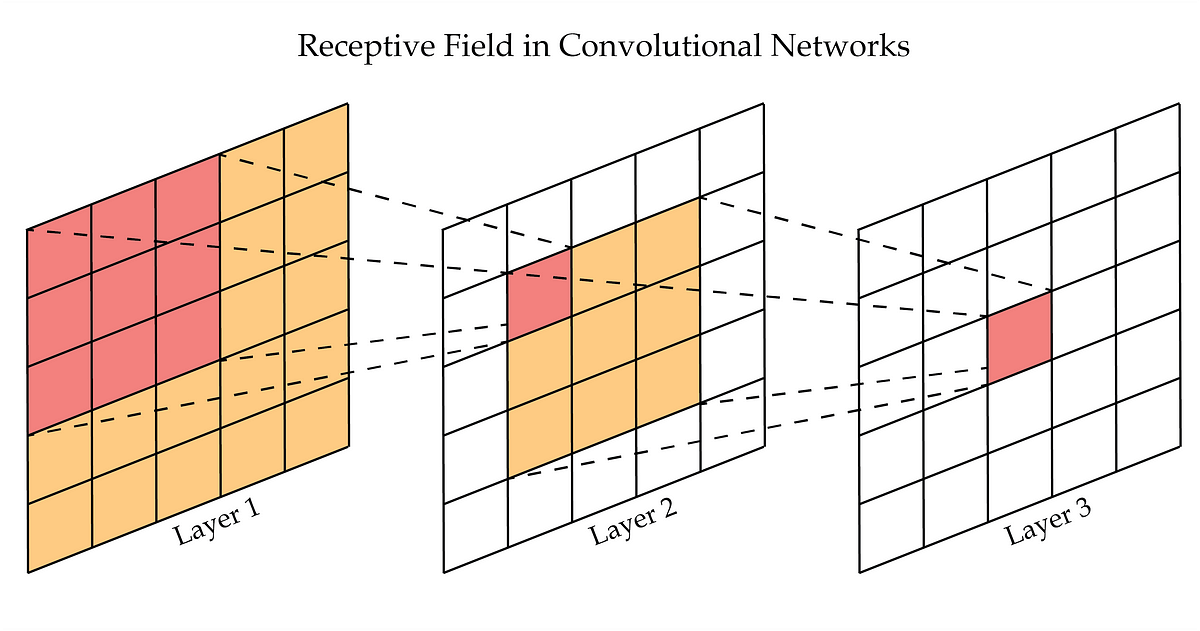
\includegraphics[width=0.75\textwidth]{figure/receptive_field.png}
    \caption{Rappresentazione del receptive field, su tre layer}
    \label{fig:recp_field}
\end{figure}
Considerando $L$ come il layer in cui ci troviamo e $K$ come il numero di dimensione del filtro, possiamo calcolare il Receptive Field ($R$), nel seguente modo:
\[
R = 1 + L \cdot (K - 1)
\]
Dunque possiamo arrivarci intuitivamente, che per ottenere una visione globale dell'immagine che stiamo analizzando, avremo bisogno di numerosi layer convoluzionali.
\section{Pooling Layer}

I livelli di \textit{Pooling} sono tipicamente interposti tra strati convoluzionali all'interno delle reti neurali convoluzionali (CNN). La loro funzione principale è quella di ridurre progressivamente la dimensione spaziale delle mappe di attivazione, attraverso un processo di \textit{downsampling}. Questo consente di diminuire il numero di parametri e il carico computazionale della rete, mitigare il rischio di overfitting e favorire l’invarianza a piccole traslazioni dell’input. Le operazioni di pooling più comuni includono:
\begin{itemize}
    \item \textbf{Max Pooling}: seleziona il valore massimo all'interno di una finestra locale (kernel) sull'immagine di input;
    \item \textbf{Average Pooling}: calcola la media dei valori nella regione coperta dal kernel;
    \item \textbf{Sum Pooling}: somma tutti i valori nella regione considerata;
\end{itemize}

Attraverso il pooling si ottiene una rappresentazione più compatta delle mappe di caratteristiche, preservando le informazioni più salienti. Questo processo di sottocampionamento permette alla rete di concentrarsi sulle caratteristiche più significative, riducendo al contempo la sensibilità a piccole variazioni locali. Combinando in modo efficace strati convoluzionali e di pooling, una CNN è in grado di apprendere progressivamente rappresentazioni gerarchiche dell’input, rilevando strutture sempre più complesse come bordi, texture, oggetti o intere scene. Infine, l’output dello strato convoluzionale finale viene \textit{appiattito} in un vettore monodimensionale, che viene successivamente fornito a uno o più strati completamente connessi (\textit{fully connected}) per eseguire il compito di classificazione.

\begin{figure}[ht]
    \centering
    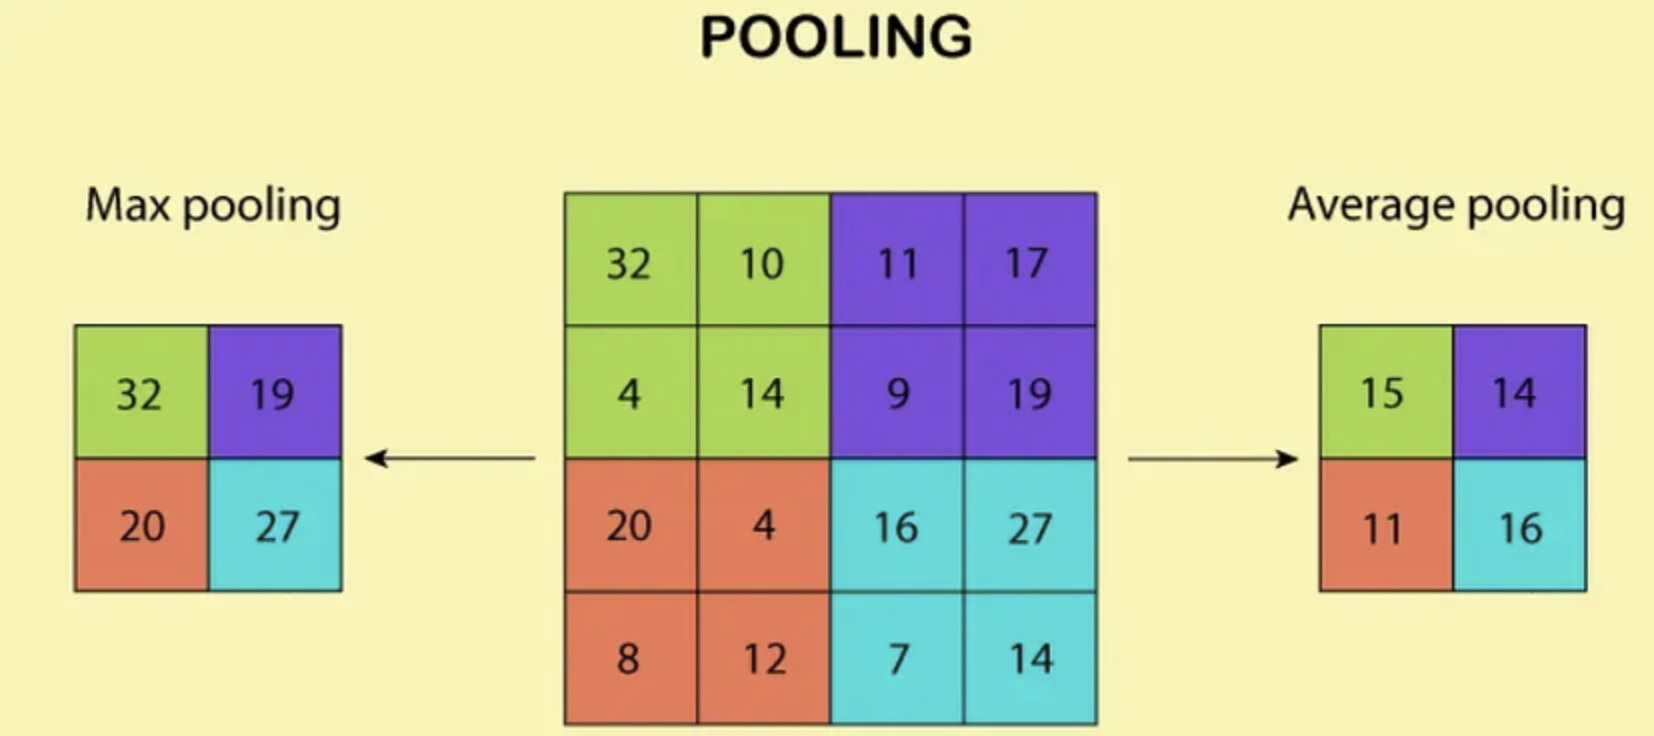
\includegraphics[width=0.55\textwidth]{figure/Pooling.png}
    \caption{Effetto del pooling applicato con kernel $2 \times 2$ e stride 2: a sinistra, il valore massimo selezionato per ciascuna finestra (Max Pooling); a destra, la media dei valori nella stessa finestra (Average Pooling).}
    \label{fig:pooling}
\end{figure}

\section{Conclusioni}

Le reti neurali convoluzionali (CNN) sfruttano in modo efficiente la struttura spaziale delle immagini attraverso tre principi fondamentali: la connettività locale, la condivisione dei pesi mediante l’impiego di filtri convoluzionali, e l’organizzazione gerarchica dei livelli. Questi elementi architetturali consentono una significativa riduzione del numero di parametri, migliorano la capacità di generalizzazione del modello e rendono la rete scalabile su immagini di grandi dimensioni. L’uso della connettività locale permette di concentrarsi su porzioni limitate dell’input, mentre la condivisione dei pesi garantisce l’invarianza traslazionale e riduce il costo computazionale. Al termine della sequenza di strati convoluzionali e di pooling, le mappe di attivazione vengono appiattite e passate a uno o più strati completamente connessi (\textit{fully connected layers}), i quali svolgono la fase finale di classificazione. Questo approccio modulare e gerarchico rende le CNN particolarmente adatte a compiti complessi di riconoscimento visivo, come dimostrato in molteplici contesti applicativi già trattati in corsi precedenti.

\begin{figure}[ht]
    \centering
    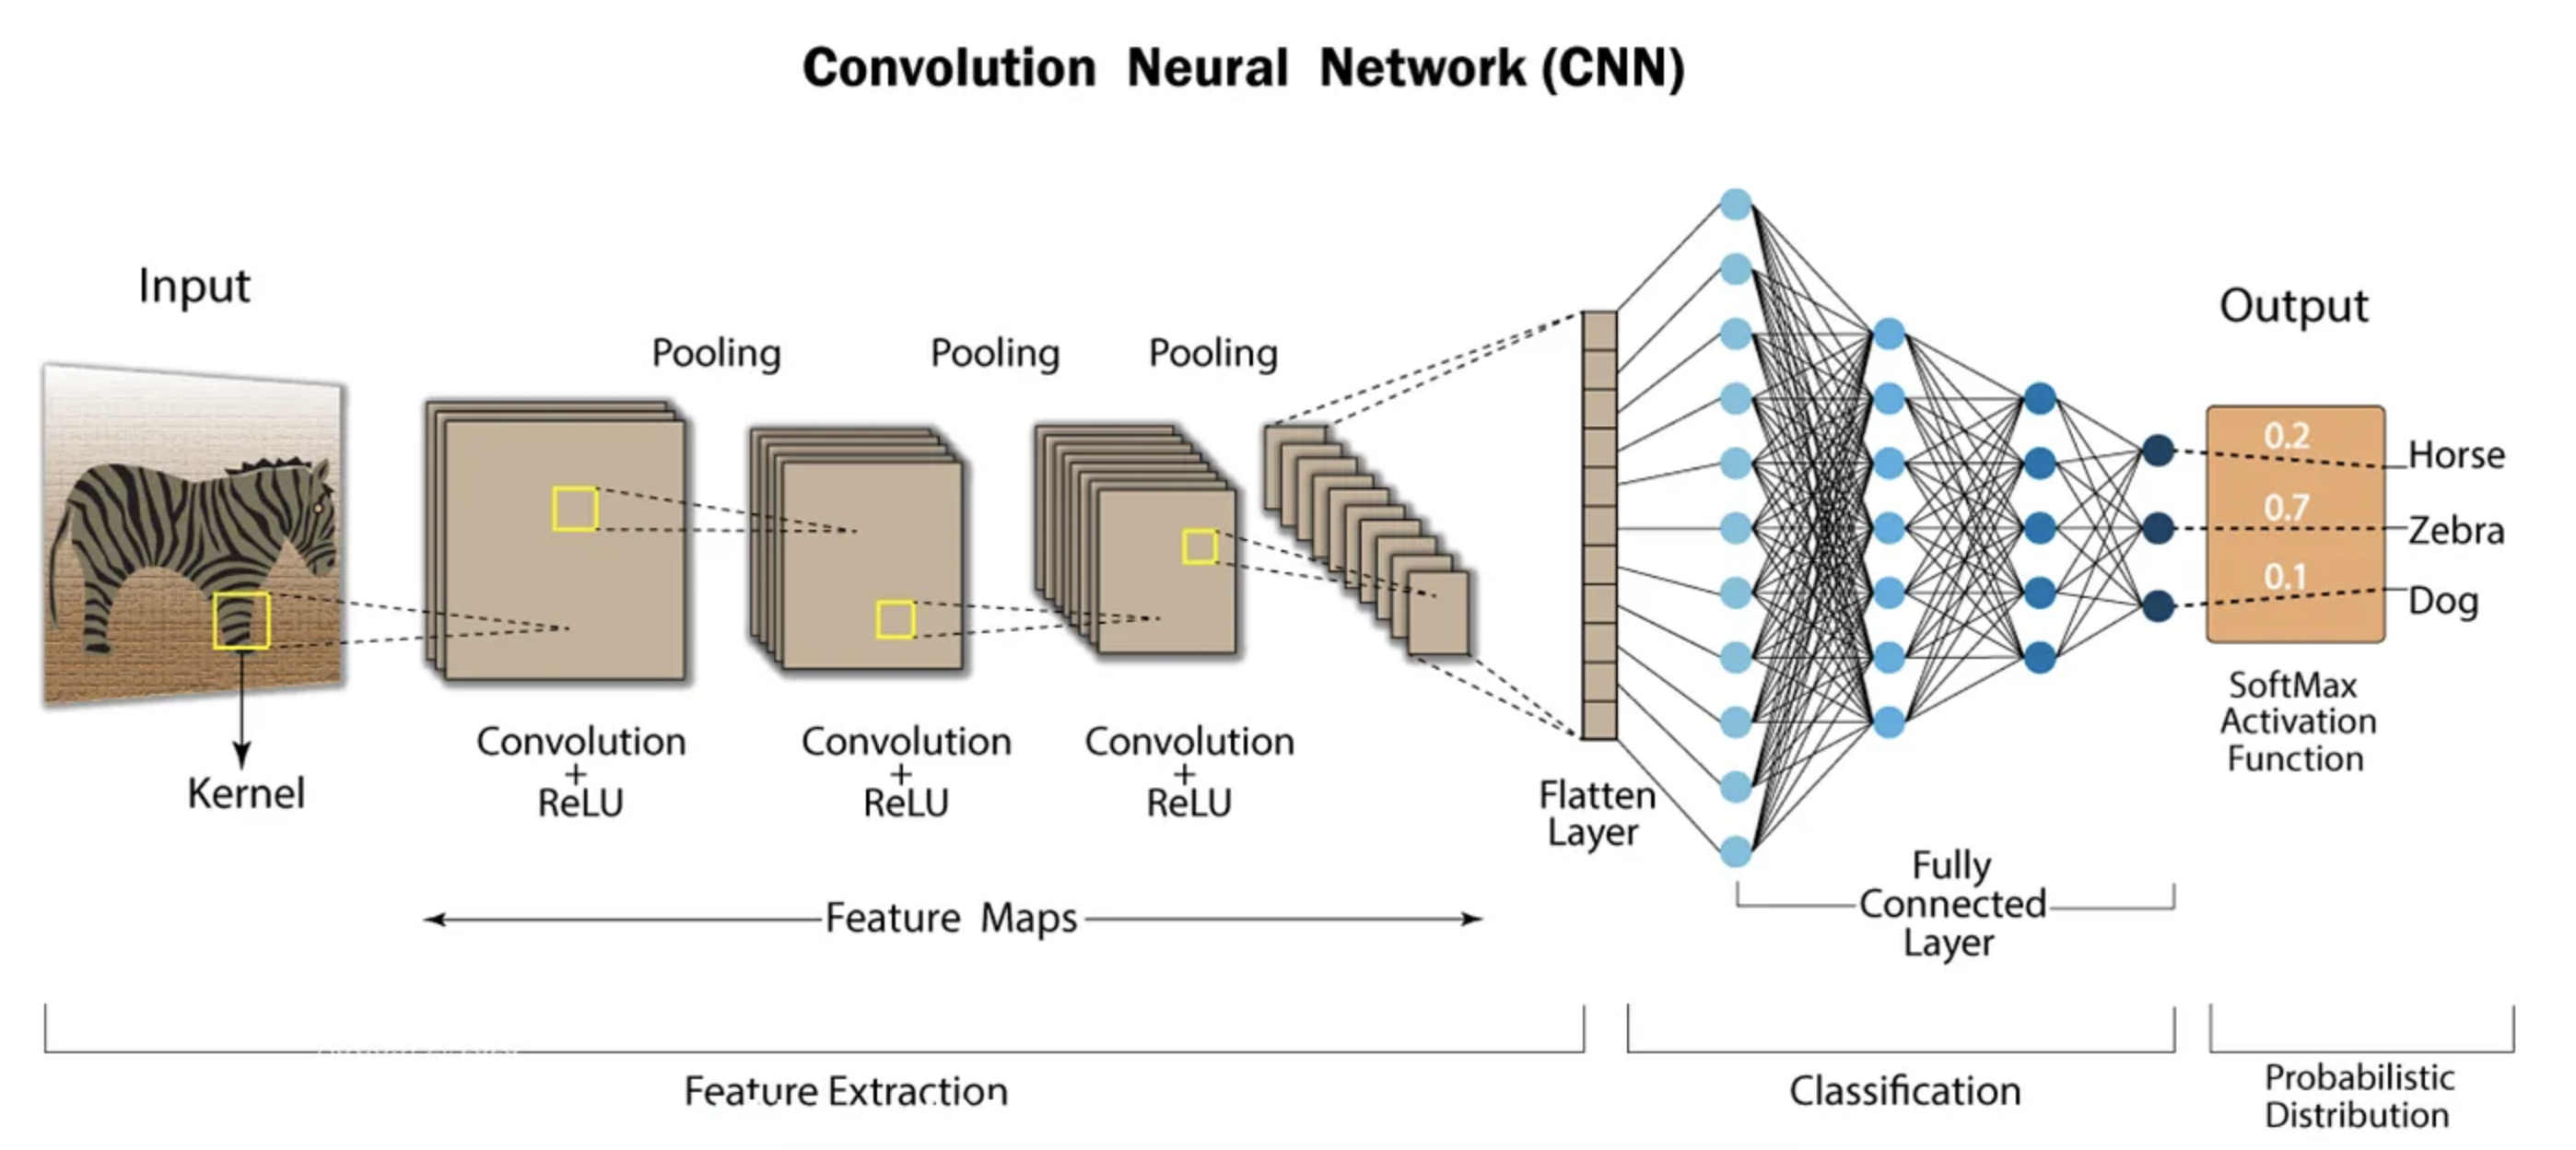
\includegraphics[width=\textwidth]{figure/ConvNN.png}
    \caption{Rappresentazione schematica di una rete neurale convoluzionale. Ogni livello svolge un’operazione distinta, contribuendo all’estrazione progressiva delle caratteristiche rilevanti dall’immagine.}
    \label{fig:ConvNN}
\end{figure}


\begin{table}[ht]
    \centering
    \caption{Confronto tra reti convoluzionali (CNN) e reti completamente connesse (Dense)}
    \label{tab:cnn_vs_dense}
    \begin{adjustbox}{width=\textwidth}
    \begin{tabular}{p{4.5cm}|p{4.5cm}|p{4.5cm}}
        \hline
        \textbf{Caratteristica} & \textbf{Reti Dense} & \textbf{Reti Convoluzionali} \\
        \hline
        Architettura & Ogni neurone connesso a tutti gli altri & Connettività locale tra neuroni \\
        \hline
        Numero di parametri & Elevato, cresce rapidamente con la dimensione dell’input & Ridotto grazie alla condivisione dei pesi \\
        \hline
        Efficienza computazionale & Bassa per immagini ad alta risoluzione & Alta, grazie all’uso di kernel \\
        \hline
        Invarianza traslazionale & Non intrinseca & Intrinseca grazie ai filtri convoluzionali \\
        \hline
        Adattabilità alle immagini & Limitata, richiede preprocessing intenso & Alta, adatte all’elaborazione visiva diretta \\
        \hline
        Capacità di generalizzazione & Tende a overfittare su dataset piccoli & Migliore grazie al minor numero di parametri \\
        \hline
    \end{tabular}
    \end{adjustbox}
\end{table}
